\documentclass[lettersize,journal]{IEEEtran}
\usepackage{amsmath,amsfonts}
\usepackage{algorithmic}
\usepackage{array}
\usepackage[caption=false,font=normalsize,labelfont=sf,textfont=sf]{subfig}
\usepackage{textcomp}
\usepackage{stfloats}
\usepackage{url}
\usepackage{verbatim}
\usepackage{graphicx}
%\graphicspath{{Images/}}
\hyphenation{op-tical net-works semi-conduc-tor IEEE-Xplore}
\def\BibTeX{{\rm B\kern-.05em{\sc i\kern-.025em b}\kern-.08em
    T\kern-.1667em\lower.7ex\hbox{E}\kern-.125emX}}
\usepackage{balance}
\begin{document}
\title{Group Introduction}

		\author{Yicong Chen,~\IEEEmembership{Postgraduate,~XDU,}
		Shunli~Tian,~\IEEEmembership{Postgraduate,~XDU,}
		Zhengxi~Guo,~\IEEEmembership{Postgraduate,~XDU,}
	
		and~Zhenyuan~Liu,~\IEEEmembership{Postgraduate,~XDU}% <-this % stops a space
\thanks{Manuscript created October, 2020; This work was developed by the IEEE Publication Technology Department. This work is distributed under the \LaTeX \ Project Public License (LPPL) ( http://www.latex-project.org/ ) version 1.3. A copy of the LPPL, version 1.3, is included in the base \LaTeX \ documentation of all distributions of \LaTeX \ released 2003/12/01 or later. The opinions expressed here are entirely that of the author. No warranty is expressed or implied. User assumes all risk.}}

\markboth{Journal of \LaTeX\ Class Files,~Vol.~18, No.~9, September~2020}%
{How to Use the IEEEtran \LaTeX \ Templates}

\maketitle

\begin{abstract}
This is a brief introduction to team members.
\end{abstract}



\section{Team member}
\IEEEPARstart{A}{t} the end of the first class, we completed the formation of a four person group. At the same time, according to recommended basic structure for a repository in the professor's paper, we build our own git repository. The following is the self introduction of the four members. 



\begin{IEEEbiography}[{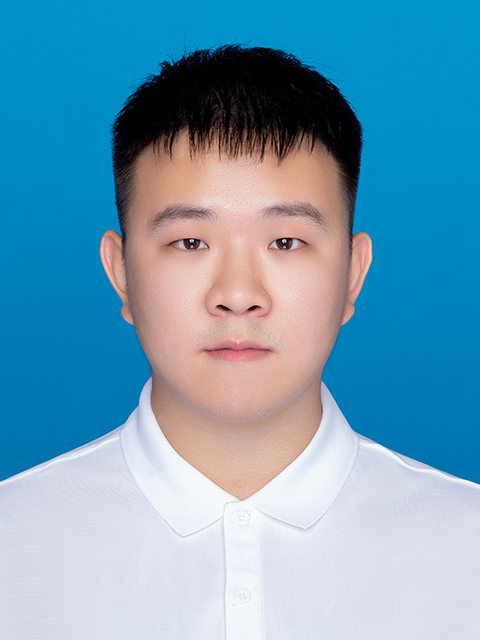
\includegraphics[width=1in,height=1.25in,clip,keepaspectratio]{D:/TeXstudio/SAR/lesson1/Images/JPG/CYC.jpg}}]{Yicong Chen}
(Postgraduate,~XDU)received the B.Sc. degree in Communication Engineering from the Ningbo University, Ningbo, in 2017.He is optimistic and positive, has working experience in the student union, has cultivated a good sense of teamwork, has participated in mathematical modeling competitions, and has a certain foundation of programming modeling.His main research direction is remote sensing image processing and analysis.\end{IEEEbiography}

\begin{IEEEbiography}[{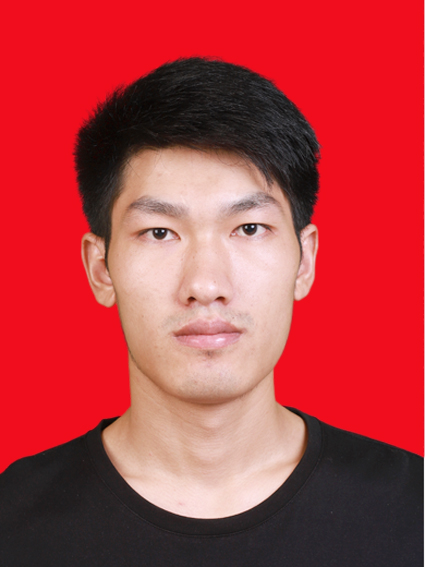
\includegraphics[width=1in,height=1.25in,clip,keepaspectratio]{D:/TeXstudio/SAR/lesson1/Images/JPG/TSL.jpg}}]{Shunli Tian}
	(Postgraduate,~XDU)comes from Yongcheng City, Henan Province.I am now studying computer Science and Technology in School of Artificial Intelligence, Xidian University.My current research direction is hyperspectral image processing.\end{IEEEbiography}

\begin{IEEEbiography}[{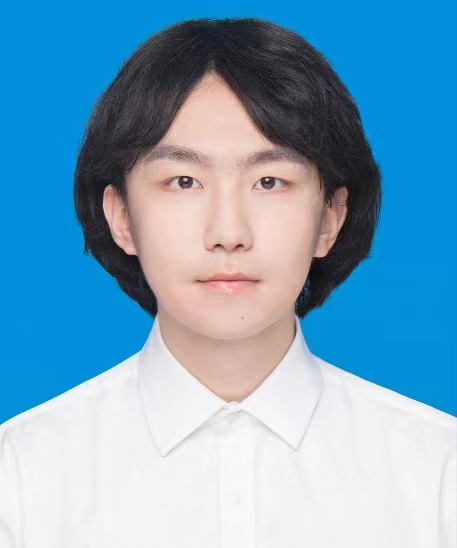
\includegraphics[width=1in,height=1.25in,clip,keepaspectratio]{D:/TeXstudio/SAR/lesson1/Images/JPG/GZX.jpg}}]{Zhengxi Guo}
	(Postgraduate,~XDU)from Xi'an, Shaanxi, is studying computer science and technology in the School of Artificial Intelligence, Xidian University, and his research direction is sar image target detection.\end{IEEEbiography}

\begin{IEEEbiography}[{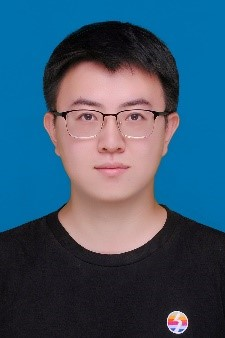
\includegraphics[width=1in,height=1.25in,clip,keepaspectratio]{D:/TeXstudio/SAR/lesson1/Images/JPG/ZYL.jpg}}]{Zhenyuan Liu}
	(Postgraduate,~XDU)graduated from the UESTC with a major in electromagnetic field and wireless technology in 2018. Have three years of work experience on pcb layout and hardware testing. The current research direction is FPGA based deep neural network design and implementation.\end{IEEEbiography}

\end{document}


